\section{Envelope Equivariant Graph Policy with Neighborhood Proximal Allocation (EGP-NPA)}\label{sec:method}

\subsection{Chiral Rotation- and Permutation-Equivariant One-Hop GNN Residual Nominal Policy}\label{subsec:gnn-arch}
To break the collinear deadlock identified in Remark~\ref{rem:two-conditions} without hand-crafting global topological potentials, we construct a distributed residual nominal policy over the one-hop directed communication graph $\mathcal G_{\mathrm c}(\bp_k)=(\mathcal V,\mathcal E_k)$ at $t_k=k\Delta t$ ($R_{\mathrm{sense}}=2.50\ \mathrm m$).

Feeding raw Cartesian coordinates $\bp_{i,k},\bg_i$ into a neural network violates Euclidean rigid-body invariance, causing identical relative formations rotated or translated in the workspace to produce inconsistent actions \cite{satorras2021egnn}. For each robot $i\in\mathcal V$, we construct a local target orthonormal frame using $\hat{\be}_{i,k}=\be_{i,k}/\max(\norm{\be_{i,k}}_2,10^{-9})$ and $\bJ\hat{\be}_{i,k}$, together with a smooth goal-vanishing factor $\sigma_{i,k}=\min(1,\norm{\be_{i,k}}_2/r_0)$ ($r_0=0.10\ \mathrm m$) to remove directional singularity as $\be_{i,k}\to\boldsymbol 0$. For each directed edge $(i,j)\in\mathcal E_k$, we construct a local edge orthonormal frame using $\hat{\br}_{ij,k}=(\bp_{j,k}-\bp_{i,k})/d_{ij,k}$ and $\bJ\hat{\br}_{ij,k}$.

Let $\bu_{i,k-1}$ be the previous executed velocity, $\boldsymbol\delta_{i,k-1}=\bu_{i,k-1}-\Pi_{\mathcal U_i}(\bu_{i,k-1}^{\mathrm{nom}})$ the filter velocity modification, $\boldsymbol\mu_{i,k-1}$ the KKT dual multiplier vector (shadow prices) from the single-robot refit QP \eqref{eq:refit-one}, $s_{i0,k-1}$ the spectral quota, and $\boldsymbol\varpi_{e,k-1}=[\varpi_{ij,0,k-1},\varpi_{ij,1,k-1}]^{\top}$ the binary edge ledger on $e=\{i,j\}$. Define the one-hop closed-neighborhood conflict memory $m_{i,k}=\max\bigl(\gamma_m m_{i,k-1},\max_{j\in\mathcal N_{i,k}^+}c_{j,k-1}\bigr)$ and gate $\gamma_{i,k}^{\mathrm{gate}}=\tanh(\beta_m m_{i,k})\in[0,1)$ ($\gamma_m=0.97,\beta_m=4.0$; $c_{j,k-1}=\norm{\boldsymbol\mu_{j,k-1}}_2$ gives the shadow-price gate $\gamma_{i,k}^{\mathrm{gate},\mu}$, while $c_{j,k-1}=\norm{\boldsymbol\delta_{j,k-1}}_2$ gives the intervention gate $\gamma_{i,k}^{\mathrm{gate,int}}$). The rotation-invariant node feature $\boldsymbol x_{i,k}=\col(\boldsymbol x_{i,k}^{\mathrm{geom}},\boldsymbol x_{i,k}^{\mathrm{alg}})\in\mathbb R^{17}$ and directed edge feature $\boldsymbol e_{ij,k}^{\mathrm{feat}}=\col(\boldsymbol e_{ij,k}^{\mathrm{geom}},\boldsymbol e_{ij,k}^{\mathrm{alg}})\in\mathbb R^{20}$ are constructed as:
\begin{equation}
\begin{split}
 \boldsymbol x_{i,k}^{\mathrm{geom}}&=\Big[\min(\norm{\be_{i,k}}_2,4),\ \mathbb I(\norm{\be_{i,k}}_2<\varepsilon_g),\ \gamma_{i,k}^{\mathrm{gate}},\\
 &\quad\ \tfrac{\norm{\bu_{i,k-1}}_2}{U},\ \tfrac{\bu_{i,k-1}^{\top}\hat{\be}_{i,k}}{U}\sigma_{i,k},\ \tfrac{\bu_{i,k-1}^{\top}\bJ\hat{\be}_{i,k}}{U}\sigma_{i,k},\\
 &\quad\ \tfrac{\norm{\boldsymbol\delta_{i,k-1}}_2}{U},\ \tfrac{\boldsymbol\delta_{i,k-1}^{\top}\hat{\be}_{i,k}}{U}\sigma_{i,k},\ \tfrac{\boldsymbol\delta_{i,k-1}^{\top}\bJ\hat{\be}_{i,k}}{U}\sigma_{i,k},\\
 &\quad\ \tfrac{\lambda_2(\bL(\bp_k))-\lr}{\lr},\ \tfrac{|\mathcal N_{i,k}|}{8},\ \min_{j\in\mathcal N_{i,k}}(d_{ij,k}-\ds)\Big]^{\top},
\end{split}\label{eq:node-geom}
\end{equation}
\begin{equation}
\begin{split}
 \boldsymbol e_{ij,k}^{\mathrm{geom}}&=\Big[\tfrac{d_{ij,k}}{R_{\mathrm{sense}}},\ \clip(d_{ij,k}-\ds,0,1.5),\ \hat{\br}_{ij,k}^{\top}\hat{\be}_{i,k}\sigma_{i,k},\\
 &\quad\ \hat{\br}_{ij,k}^{\top}\bJ\hat{\be}_{i,k}\sigma_{i,k},\ \hat{\br}_{ij,k}^{\top}\hat{\be}_{j,k}\sigma_{j,k},\ \hat{\br}_{ij,k}^{\top}\bJ\hat{\be}_{j,k}\sigma_{j,k},\\
 &\quad\ \min(\norm{\be_{j,k}}_2,4),\ \hat{\be}_{i,k}^{\top}\hat{\be}_{j,k}\sigma_{i,k}\sigma_{j,k},\\
 &\quad\ (\bJ\hat{\be}_{i,k})^{\top}\hat{\be}_{j,k}\sigma_{i,k}\sigma_{j,k},\ \tfrac{(\bu_{j,k-1}-\bu_{i,k-1})^{\top}\hat{\br}_{ij,k}}{U},\\
 &\quad\ \tfrac{(\bu_{j,k-1}-\bu_{i,k-1})^{\top}\bJ\hat{\br}_{ij,k}}{U},\ \gamma_{j,k}^{\mathrm{gate}},\ \tfrac{\norm{\boldsymbol\delta_{j,k-1}}_2}{U}\Big]^{\top},
\end{split}\label{eq:edge-geom}
\end{equation}
\begin{equation}
\begin{split}
 \boldsymbol x_{i,k}^{\mathrm{alg}}&=\Big[\ln(1+|\mu_{i0,k-1}|),\ \ln\big(1+\textstyle\sum_{j\ne i}|\mu_{ij,k-1}|\big),\\
 &\quad\ \clip\big(\tfrac{s_{i0,k-1}}{\bar\nu_{i0,k}},-3,3\big),\ \ln(1+\norm{\boldsymbol\mu_{i,k-1}}_2),\\
 &\quad\ \clip\big(\tfrac{U\norm{\boldsymbol a_{i0,k}}_2-b_{i0,k}-s_{i0,k-1}}{\bar\nu_{i0,k}},-3,3\big)\Big]^{\top},\\
 \boldsymbol e_{ij,k}^{\mathrm{alg}}&=\Big[\ln(1+|\mu_{ij,k-1}|),\ \ln(1+|\mu_{ji,k-1}|),\\
 &\quad\ \tanh(2\varpi_{ij,0,k-1}),\ \tanh(2\varpi_{ij,1,k-1}),\\
 &\quad\ |\tilde\phi_{i,k}-\tilde\phi_{j,k}|,\ \norm{\widetilde{\boldsymbol\Phi}_{i,k}-\widetilde{\boldsymbol\Phi}_{j,k}}_2,\ \widetilde{\boldsymbol\Phi}_{i,k}^{\top}\widetilde{\boldsymbol\Phi}_{j,k}\Big]^{\top},
\end{split}\label{eq:alg-feat}
\end{equation}
where $\bar\nu_{i0,k}=U\norm{\boldsymbol a_{i0,k}}_2+|b_{i0,k}|+10^{-3}$ normalizes the spectral row, and $\tilde\phi_{i,k}=\sqrt{N}\phi_{i,k}$, $\widetilde{\boldsymbol\Phi}_{i,k}=\sqrt{N}\boldsymbol\Phi_{i,k}\in\mathbb R^2$ are unit-RMS normalized spectral states satisfying $\frac1N\sum_{i=1}^N\tilde\phi_{i,k}^2=1$.

A parameter-shared $L_{\mathrm{gnn}}=2$-layer message-passing GNN encodes $\boldsymbol h_i^{(0)}=\phi_{\mathrm{enc}}(\boldsymbol x_{i,k})\in\mathbb R^{d_h}$ ($d_h=64$) and performs one-hop message passing with mean--max dual aggregation across layers $\ell\in\{1,\dots,L_{\mathrm{gnn}}\}$:
\begin{equation}
\begin{split}
 \boldsymbol m_{ij}^{(\ell)}&=\phi_{\mathrm{msg}}^{(\ell)}\big(\col(\boldsymbol h_i^{(\ell-1)},\boldsymbol h_j^{(\ell-1)},\boldsymbol e_{ij,k}^{\mathrm{feat}})\big),\quad\forall (i,j)\in\mathcal E_k,\\
 \bar{\boldsymbol m}_i^{(\ell)}&=\frac{1}{\max(|\mathcal N_{i,k}|,1)}\sum_{j\in\mathcal N_{i,k}}\boldsymbol m_{ij}^{(\ell)},\quad
 \hat{\boldsymbol m}_i^{(\ell)}=\max_{j\in\mathcal N_{i,k}}\boldsymbol m_{ij}^{(\ell)},\\
 \boldsymbol h_i^{(\ell)}&=\operatorname{LN}^{(\ell)}\!\Big(\boldsymbol h_i^{(\ell-1)}+\phi_{\mathrm{upd}}^{(\ell)}\big(\col(\boldsymbol h_i^{(\ell-1)},\bar{\boldsymbol m}_i^{(\ell)},\hat{\boldsymbol m}_i^{(\ell)})\big)\Big),
\end{split}\label{eq:gnn-layer}
\end{equation}
where $\phi_{\mathrm{enc}},\phi_{\mathrm{msg}}^{(\ell)},\phi_{\mathrm{upd}}^{(\ell)}$ are Multi-Layer Perceptrons (MLPs) with $\operatorname{SiLU}$ activations and $\operatorname{LN}^{(\ell)}$ denotes Layer Normalization. Output heads $\phi_{\mathrm{node}}$ and $\phi_{\mathrm{edge}}$ produce bounded scalar action coefficients:
\begin{equation}
\begin{split}
 (\omega_{i,k}^\theta,r_{i,k}^\theta)&=\clip\big(\phi_{\mathrm{node}}(\boldsymbol h_i^{(L_{\mathrm{gnn}})}),-1,1\big),\\
 \psi_{ij,k}^\theta&=\clip\big(\phi_{\mathrm{edge}}(\col(\boldsymbol h_i^{(L_{\mathrm{gnn}})},\boldsymbol h_j^{(L_{\mathrm{gnn}})},\boldsymbol e_{ij,k}^{\mathrm{feat}})),-1,1\big),
\end{split}\label{eq:action-heads}
\end{equation}
which synthesize the planar nominal velocity of robot $i$:
\begin{equation}
\begin{split}
 \bu_{i,k}^{\mathrm{nom}}(\bp_k;\theta)&=-\be_{i,k}+\gamma_{i,k}^{\mathrm{eff}}\br_{i,k}^\theta(\bp_k),\\
 \br_{i,k}^\theta(\bp_k)&=A_{\mathrm{rot}}\omega_{i,k}^\theta\bJ\be_{i,k}+A_{\mathrm{rad}}r_{i,k}^\theta\be_{i,k}\\
 &\quad+\frac{A_\psi U}{\max(|\mathcal N_{i,k}|,1)}\sum_{j\in\mathcal N_{i,k}}\psi_{ij,k}^\theta\frac{\bp_{i,k}-\bp_{j,k}}{d_{ij,k}},
\end{split}\label{eq:nominal-law}
\end{equation}
where $\gamma_{i,k}^{\mathrm{eff}}\in[0,1)$ is the composite envelope gate (Section~\ref{subsec:envelope}) and $A_{\mathrm{rot}}=2.0\ \mathrm s^{-1},A_{\mathrm{rad}}=1.5\ \mathrm s^{-1},A_\psi=2.0$. Here $-\be_{i,k}$ provides baseline goal attraction; $A_{\mathrm{rot}}\omega_{i,k}^\theta\bJ\be_{i,k}$ generates tangential circulation perpendicular to the line-of-sight to break head-on collinear symmetry; $A_{\mathrm{rad}}r_{i,k}^\theta\be_{i,k}$ modulates radial approach speed; and $\sum_{j\in\mathcal N_{i,k}}\psi_{ij,k}^\theta(\bp_{i,k}-\bp_{j,k})/d_{ij,k}$ provides pairwise repulsive bias along neighbor links.

\begin{proposition}[$\mathrm{SO}(2)\ltimes\mathbb R^2$ and Permutation Equivariance and Chiral Symmetry Breaking]\label{prop:equivariance}
For any network parameters $\theta$, any rotation matrix $\boldsymbol R\in\mathrm{SO}(2)$, translation $\boldsymbol c\in\mathbb R^2$, and $N\times N$ permutation matrix $\boldsymbol P_\pi$, let $(\tilde\bp_i,\tilde\bg_i,\tilde\bu_{i,k-1})=(\boldsymbol R\bp_i+\boldsymbol c,\boldsymbol R\bg_i+\boldsymbol c,\boldsymbol R\bu_{i,k-1})$. Then the nominal control field \eqref{eq:nominal-law} satisfies:
\begin{equation}
\begin{split}
 \bu_{i,k}^{\mathrm{nom}}(\tilde\bp_k,\tilde\bg;\theta)&=\boldsymbol R\bu_{i,k}^{\mathrm{nom}}(\bp_k,\bg;\theta),\\
 \bu_k^{\mathrm{nom}}\big((\boldsymbol P_\pi\otimes\I_2)\bp_k,(\boldsymbol P_\pi\otimes\I_2)\bg\big)&=(\boldsymbol P_\pi\otimes\I_2)\bu_k^{\mathrm{nom}}(\bp_k,\bg).
\end{split}\label{eq:equiv-prop}
\end{equation}
Furthermore, if \eqref{eq:nominal-law} is constrained to be equivariant under the full orthogonal group $\mathrm{O}(2)$ (including planar reflections $\boldsymbol M\in\mathrm{O}(2)\setminus\mathrm{SO}(2)$ with $\det\boldsymbol M=-1$), then on any encounter configuration that is mirror-symmetric across $\hat{\be}_{i,k}$, the tangential circulation coefficient necessarily collapses to $\omega_{i,k}^\theta\equiv 0$.
\end{proposition}
\begin{proof}
Under $\mathrm{SO}(2)\ltimes\mathbb R^2$, $\tilde\be_{i,k}=\boldsymbol R\be_{i,k}$ and $\tilde\bp_{ij,k}=\boldsymbol R\bp_{ij,k}$. Since $\boldsymbol R\in\mathrm{SO}(2)$ preserves Euclidean norms and inner products and commutes with $\bJ$ ($\boldsymbol R\bJ=\bJ\boldsymbol R$), all scalar features in \eqref{eq:node-geom}--\eqref{eq:alg-feat} and action coefficients $(\omega_{i,k}^\theta,r_{i,k}^\theta,\psi_{ij,k}^\theta)$ are strictly invariant. Substituting into \eqref{eq:nominal-law} and using $\boldsymbol R\bJ\be_{i,k}=\bJ\boldsymbol R\be_{i,k}$ yields the first identity; permutation equivariance follows from parameter sharing and symmetric mean/max aggregation in \eqref{eq:gnn-layer}. Conversely, any reflection $\boldsymbol M\in\mathrm{O}(2)\setminus\mathrm{SO}(2)$ anticommutes with $\bJ$ ($\boldsymbol M\bJ=-\bJ\boldsymbol M$). On a state mirror-symmetric under $\boldsymbol M$ ($\boldsymbol M\be_{i,k}=\be_{i,k}$), $\mathrm{O}(2)$ equivariance requires $\boldsymbol M\bu_{i,k}^{\mathrm{nom}}=\bu_{i,k}^{\mathrm{nom}}$, whose projection along $\bJ\be_{i,k}$ forces $-\omega_{i,k}^\theta=\omega_{i,k}^\theta\implies\omega_{i,k}^\theta\equiv 0$.
\end{proof}

\subsection{Closed-Neighborhood Dynamic Quota Shield and Cooperative Yielding of Stationary Neighbors}\label{subsec:npa-yield}
The nominal velocity $\bu_{i,k}^{\mathrm{nom}}$ is filtered by the $B$-round closed-neighborhood block NPA shield $L$ (Section~\ref{subsec:npa-prelim}) and verified by the exact rational ZOH segment certificate (Theorem~\ref{thm:zoh-safe}).

\begin{proposition}[Anytime Hard Safety Invariance Under Exploration and Cross-Scale Deployment]\label{prop:safety}
Suppose $\bp_0\in\mathcal S$ and $b_{ia,k}\le 0$. Then for arbitrary policy parameters $\theta$ (including noisy policies during training exploration and zero-shot deployment to any team size $N$) and any finite number of allocation rounds $B\ge 0$, the closed-loop continuous trajectory $\bp(t)$ satisfies $d_{ij}(t)\ge\ds$ ($\forall i<j$), $\lambda_2(\bL(\bp(t)))\ge\lr$, $\bu_i(t)\in\mathcal U_i$, and $\bp(t)\in\mathcal X$ for all $t\ge 0$.
\end{proposition}
\begin{proof}
By the antisymmetric edge-ledger construction \eqref{eq:edge-ledger}, Stage~1 revocation and one-hop local settlement guarantee $\sum_{i\in\mathcal V_a}s_{ia,k}^{(0)}=0$ and single-robot feasibility \eqref{eq:refit-one}. Each block QP \eqref{eq:block-qp} in Stage~2 preserves zero-sum quotas via $\sum_{q\in\mathcal N_{i,k}^+}w_q=0$ and $\sigma_{q,e}t_e+\sigma_{m,e}t_e=0$, and the convex combination \eqref{eq:convex-commit} maintains feasibility of $(\bu_k^{(B)},\boldsymbol s_k^{(B)})$ for all coupled constraints \eqref{eq:coupled-rows}. Combined with adaptive ZOH step-halving under Theorem~\ref{thm:zoh-safe}, $\bp(t)\in\mathcal S$ holds for all $t\ge 0$ by induction.
\end{proof}

We next prove algebraically why dynamic quota transfer $t_e$ in \eqref{eq:block-qp} is the exact mechanism that unfreezes outer stationary neighbors, whereas static equal allocation ($B=0$) induces artificial freezing.

\begin{proposition}[Cooperative Unfreezing of Stationary Blocking Neighbors via Dynamic Quota Transfer]\label{prop:unfreeze}
Consider a contact pair on the safety boundary $d_{ij}=\ds$ ($b_{ia}=b_{ja}=0$) between a moving robot $i$ and a stationary target-holding neighbor $j$ ($\be_j=\boldsymbol 0,\bu_j^{\mathrm{nom}}=\boldsymbol 0$), with unit contact normal $\boldsymbol n_{ij}=(\bp_i-\bp_j)/\ds$. Suppose the GNN residual policy \eqref{eq:nominal-law} generates a lateral bypass nominal velocity for robot $i$ with strictly positive normal intrusion $\delta_n:=-\boldsymbol n_{ij}^{\top}\bu_i^{\mathrm{nom}}>0$ (unsaturated):
\begin{enumerate}
 \item \textbf{Artificial freezing under static equal splitting ($B=0,s_{ia}=s_{ja}\equiv 0$):} The decoupled constraints reduce to $-2\ds\boldsymbol n_{ij}^{\top}\bu_i\le 0$ and $2\ds\boldsymbol n_{ij}^{\top}\bu_j\le 0$. Since $\bu_j^{\mathrm{nom}}=\boldsymbol 0$ is feasible for node $j$, $\bu_j^{\mathrm{stat}}=\boldsymbol 0$ (stationary neighbor remains frozen) while robot $i$'s normal component is truncated to zero ($-\boldsymbol n_{ij}^{\top}\bu_i^{\mathrm{stat}}=0$).
 \item \textbf{Quota transfer and cooperative yielding under closed-neighborhood dynamic allocation ($B\ge 1$):} In the two-node contact block subproblem of \eqref{eq:block-qp} starting from zero quotas, the unique optimal pairwise quota transfer $t_{ij}^\star$, normal advance speed $-\boldsymbol n_{ij}^{\top}\bu_i^\star$, and outward yielding speed $-\boldsymbol n_{ij}^{\top}\bu_j^\star$ admit the strictly positive closed-form solution:
 \begin{equation}
 \begin{split}
  |t_{ij}^\star| &= \frac{\eta\ds}{\eta+4\ds^2}\delta_n > 0,\\
  -\boldsymbol n_{ij}^{\top}\bu_i^\star &= -\boldsymbol n_{ij}^{\top}\bu_j^\star = \frac{\eta}{2(\eta+4\ds^2)}\delta_n > 0.
 \end{split}\label{eq:joint-yield}
 \end{equation}
\end{enumerate}
\end{proposition}
\begin{proof}
At $d_{ij}=\ds$, $\boldsymbol a_{ia}=-2\ds\boldsymbol n_{ij},\boldsymbol a_{ja}=2\ds\boldsymbol n_{ij},b_{ia}=b_{ja}=0$. Decompose velocities into normal components $u_{q,n}=-\boldsymbol n_{ij}^{\top}\bu_q$ (positive outward from $i$ toward $j$) and tangential components $\bu_{q,\tau}=(\I_2-\boldsymbol n_{ij}\boldsymbol n_{ij}^{\top})\bu_q$. Tangential components are unconstrained, so $\bu_{i,\tau}^\star=\bu_{i,\tau}^{\mathrm{nom}},\bu_{j,\tau}^\star=\boldsymbol 0$. Along the normal direction: (1) For $B=0,s_{ia}=s_{ja}=0$, minimizing $\frac12(u_{i,n}-\delta_n)^2$ subject to $2\ds u_{i,n}\le 0$ and $\frac12 u_{j,n}^2$ subject to $-2\ds u_{j,n}\le 0$ yields $u_{i,n}^{\mathrm{stat}}=u_{j,n}^{\mathrm{stat}}=0$. (2) In the block QP \eqref{eq:block-qp}, the normal constraints are $2\ds u_{i,n}+t_{ij}\le 0$ and $-2\ds u_{j,n}-t_{ij}\le 0$ with strictly convex cost $\frac12(u_{i,n}-\delta_n)^2+\frac12 u_{j,n}^2+\frac{1}{\eta}t_{ij}^2$. Since the unconstrained minimum $(\delta_n,0,0)$ violates $2\ds u_{i,n}+t_{ij}\le 0$, both constraints are active at optimum: $t_{ij}=-2\ds u_{i,n}=-2\ds u_{j,n}$ and $u_{i,n}^\star=u_{j,n}^\star=:v_n$. Minimizing $f(v_n)=\frac12(v_n-\delta_n)^2+\frac12 v_n^2+\frac{4\ds^2}{\eta}v_n^2$ gives $(2+\frac{8\ds^2}{\eta})v_n=\delta_n$, yielding \eqref{eq:joint-yield}.
\end{proof}

Proposition~\ref{prop:unfreeze} reveals why penalizing the normal filter modification $u_{i,n}^\star-\delta_n=-\frac{\eta+8\ds^2}{2(\eta+4\ds^2)}\delta_n\ne 0$ via a projection consistency loss $\norm{\Pi_{\mathcal U_i}(\bu_{i,k}^{\mathrm{nom}})-\operatorname{sg}(\bu_{i,k})}_2^2$ is counterproductive under dynamic quota sharing: driving $\delta_n\to 0$ eliminates the quota transfer $|t_{ij}^\star|$ in \eqref{eq:joint-yield} and deprives stationary neighbors of their outward yielding drive.

\subsection{One-Hop Closed-Neighborhood Completion Envelope and Goal Equilibrium Recovery}\label{subsec:envelope}

\begin{figure*}[t]
 \centering
 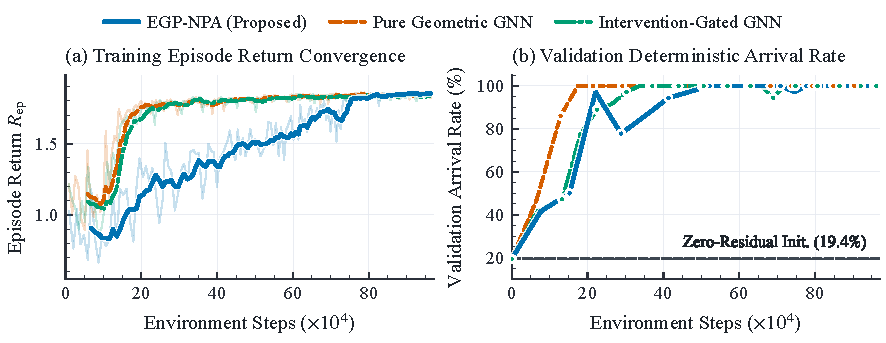
\includegraphics[width=\textwidth]{figures_en/fig2_training_curves.pdf}
 \caption{MAPPO training evolution over $9.6\times 10^5$ environment steps. (a) Episode return $R_{\mathrm{ep}}$ convergence (faint lines: raw episode returns; bold lines: moving average); (b) deterministic arrival rate on the $N=8$ validation benchmark ($36$ swap and permutation instances).}
 \label{fig:train-curves}
\end{figure*}

In \eqref{eq:nominal-law}, the tangential and radial residual terms scale with $\be_{i,k}$ and vanish as $\be_{i,k}\to\boldsymbol 0$, whereas the pairwise repulsive bias $\boldsymbol b_{i,k}^\psi=\frac{A_\psi U}{\max(|\mathcal N_{i,k}|,1)}\sum_{j\in\mathcal N_{i,k}}\psi_{ij,k}^\theta(\bp_{i,k}-\bp_{j,k})/d_{ij,k}$ is a zero-order term of unit direction vectors. On a tightly packed goal lattice with spacing $1.001\ \mathrm m$ ($1\ \mathrm{mm}$ above $\ds=1.000\ \mathrm m$), near-active contact constraints maintain $\norm{\boldsymbol\mu_{i,k-1}}_2>0$ and $\gamma_{i,k}^{\mathrm{gate}}\approx 1$, causing $\boldsymbol b_{i,k}^\psi$ to balance $-\be_{i,k}$ at $\norm{\be_{i,k}}_2\in[0.015,0.05]\ \mathrm m$ (terminal steady-state hovering).

To keep residuals active whenever any one-hop neighbor has not yet reached its goal while enforcing unconditional first-order vanishing once the entire one-hop closed neighborhood enters the goal ball, we define the \emph{One-Hop Closed-Neighborhood Completion Envelope}:
\begin{equation}
\begin{split}
 \rho_{i,k}(\bp_k)&=\tanh\!\left(\frac{\max_{j\in\mathcal N_{i,k}^+}\norm{\bp_{j,k}-\bg_j}_2}{\varepsilon_g}\right),\\
 \gamma_{i,k}^{\mathrm{eff}} &= \gamma_{i,k}^{\mathrm{gate}}\cdot\rho_{i,k}(\bp_k),
\end{split}\label{eq:envelope-def}
\end{equation}
with envelope scale $\varepsilon_g=0.05\ \mathrm m$ ($5\times$ the arrival tolerance $0.01\ \mathrm m$).

\begin{proposition}[First-Order Residual Vanishing and Goal Equilibrium Recovery]\label{prop:envelope}
Under the completion envelope \eqref{eq:envelope-def} in \eqref{eq:nominal-law}:
\begin{enumerate}
 \item \textbf{Residual preservation during cooperative transit:} Whenever there exists $j\in\mathcal N_{i,k}^+$ with $\norm{\be_{j,k}}_2\ge 3\varepsilon_g=0.15\ \mathrm m$, even if $\be_{i,k}=\boldsymbol 0$, we have $\rho_{i,k}(\bp_k)\ge\tanh(3)>0.995$.
 \item \textbf{First-order suppression near the goal and equilibrium restoration:} Let $e_{i,k}^{\max}:=\max_{j\in\mathcal N_{i,k}^+}\norm{\be_{j,k}}_2\le\norm{\be_k}_2$. Since $\tanh(z)\le z$ ($\forall z\ge 0$), $\gamma_{i,k}^{\mathrm{gate}}\in[0,1)$, and $|\omega_{i,k}^\theta|,|r_{i,k}^\theta|,|\psi_{ij,k}^\theta|\le 1$,
 \begin{equation}
 \begin{split}
  \norm{\gamma_{i,k}^{\mathrm{eff}}\br_{i,k}^\theta(\bp_k)}_2
  &\le \frac{e_{i,k}^{\max}}{\varepsilon_g}\Big[(A_{\mathrm{rot}}+A_{\mathrm{rad}})\norm{\be_{i,k}}_2+A_\psi U\Big]\\
  &=\mathcal O(\norm{\be_k}_2).
 \end{split}\label{eq:residual-bound}
 \end{equation}
 In particular, at $\bp_k=\bg$, $\rho_{i,k}(\bg)=0$ and $\bu_{i,k}^{\mathrm{nom}}(\bg;\theta)=\boldsymbol 0$ regardless of $\boldsymbol\mu_{i,k-1}$.
\end{enumerate}
\end{proposition}
\begin{proof}
Claim (1) follows from monotonicity of $\tanh(\cdot)$ since $\tanh(3)\approx 0.99505>0.995$. Claim (2) follows from $0\le\gamma_{i,k}^{\mathrm{eff}}\le\rho_{i,k}(\bp_k)\le e_{i,k}^{\max}/\varepsilon_g$ and the triangle inequality $\norm{\br_{i,k}^\theta(\bp_k)}_2\le(A_{\mathrm{rot}}+A_{\mathrm{rad}})\norm{\be_{i,k}}_2+A_\psi U$. Setting $\be_k=\boldsymbol 0$ yields $\bu_{i,k}^{\mathrm{nom}}(\bg;\theta)=\boldsymbol 0$.
\end{proof}

\subsection{Small-Scale Short-Horizon MAPPO Training and Zero-Shot Cross-Scale Deployment}\label{subsec:mappo}
Because the $B$-round block QP filter $L$ involves nonsmooth active-set switches and local settlements, backpropagating long-horizon policy gradients through the QP solver suffers from gradient singularities at multi-contact corners. We adopt a Centralized Training with Decentralized Execution (CTDE) MAPPO protocol \cite{yu2022mappo} that combines small-scale short-horizon training ($N\in\{6,\dots,10\},B=2$, validation selection on $N=8$) with large-scale multi-round zero-shot deployment ($N\in\{12,20,25\},B=8$), as summarized in Table~\ref{tab:algo1}. Training tasks are sampled on dense triangular lattices (spacing $1.001\sim 1.12\ \mathrm m$, $\lr/\lambda_2(\bp_0)\in[0.55,0.90]$, $1\sim 3$ pair swaps, 3-cycle rotations, and full permutations with random global rotation). The shared team reward at step $k$ is:
\begin{equation}
\begin{split}
 R_k &= r_{\mathrm{prog}}\frac{\sum_{i=1}^N\big(\norm{\be_{i,k}}_2-\norm{\be_{i,k+1}}_2\big)}{D_0} - r_{\mathrm{time}}\\
 &\quad + r_{\mathrm{succ}}\mathbb I\Big(\max_{i\in\mathcal V}\norm{\be_{i,k+1}}_2\le\varepsilon_{\mathrm{succ}}\Big)\\
 &\quad - \frac{r_{\mathrm{stall}}}{N}\sum_{i=1}^N\tanh\!\Big(\frac{\norm{\be_{i,k}}_2}{\varepsilon_p}\Big)\exp\!\Big(-\frac{\norm{\bu_{i,k}}_2^2}{\varepsilon_u^2}\Big)\\
 &\quad\qquad\qquad\times\ln\!\big(1+\norm{\boldsymbol\mu_{i,k}}_2^2\big),
\end{split}\label{eq:reward}
\end{equation}
where $D_0=\sum_{i=1}^N\norm{\be_{i,0}}_2$, $r_{\mathrm{prog}}=1.0$, $r_{\mathrm{time}}=10^{-3}$, $\varepsilon_{\mathrm{succ}}=0.01\ \mathrm m,r_{\mathrm{succ}}=1.0$, and the fourth term penalizes dual-blocked stagnation ($r_{\mathrm{stall}}=0.02,\varepsilon_p=0.10\ \mathrm m,\varepsilon_u=0.05\ \mathrm{m/s}$). Policy parameters $\theta$ are updated via GAE ($\gamma=0.995,\lambda_{\mathrm{GAE}}=0.95$) and clipped PPO ($\epsilon_{\mathrm{clip}}=0.20$, target KL $0.03$).

\begin{table}[htbp]
 \centering\footnotesize
 \caption{EGP-NPA Training and Zero-Shot Distributed Execution (Algorithm~1)}\label{tab:algo1}
 \renewcommand{\arraystretch}{1.10}
 \begin{tabularx}{\columnwidth}{@{}X@{}}
 \toprule
 \textbf{Phase A: Small-Scale Short-Horizon CTDE Training ($N\in\{6,\dots,10\},\ B_{\mathrm{train}}=2$)}\\
 \midrule
 1. Initialize 2-layer equivariant GNN actor $\theta$ and centralized GNN critic $\phi$;\\
 2. \textbf{for} iteration $m=1,2,\dots,M_{\max}$ \textbf{do}\\
 3. \hspace{0.8em}Sample dense triangular-lattice swap/permutation tasks ($N\in\{6,\dots,10\}$, random rotation), set $\boldsymbol\varpi_{-1}=\boldsymbol 0$;\\
 4. \hspace{0.8em}\textbf{for} step $k=0,1,\dots,K_{\max}-1$ \textbf{do}\\
 5. \hspace{1.6em}Construct invariant features $(\boldsymbol x_{i,k},\boldsymbol e_{ij,k}^{\mathrm{feat}})$ and sample noisy nominal velocity $\bu_{i,k}^{\mathrm{nom}}$ via \eqref{eq:gnn-layer}--\eqref{eq:nominal-law};\\
 6. \hspace{1.6em}Solve single-robot refit QP \eqref{eq:refit-one} (recording shadow prices $\boldsymbol\mu_{i,k}$) and apply one-hop local settlement if needed;\\
 7. \hspace{1.6em}Run $B_{\mathrm{train}}=2$ closed-neighborhood block NPA rounds \eqref{eq:block-qp}--\eqref{eq:convex-commit} and ZOH certificate (Theorem~\ref{thm:zoh-safe});\\
 8. \hspace{1.6em}Compute team reward $R_k$ via \eqref{eq:reward} and store transition in rollout buffer;\\
 9. \hspace{0.8em}\textbf{end for}\\
 10. \hspace{0.4em}Compute GAE advantages, update $(\theta,\phi)$ via clipped PPO, and save best checkpoint $\theta^\star$ on $N=8$ validation set.\\
 11. \textbf{end for}\\
 \midrule
 \textbf{Phase B: Zero-Shot Cross-Scale Decentralized Execution (Arbitrary $N$, $\theta=\theta^\star,\ B_{\mathrm{eval}}=8$)}\\
 \midrule
 12. At each step $t_k$, each robot $i\in\mathcal V$ evaluates completion envelope $\rho_{i,k}(\bp_k)=\tanh(\max_{j\in\mathcal N_{i,k}^+}\norm{\be_{j,k}}_2/\varepsilon_g)$;\\
 13. Compute deterministic GNN actions $(\omega_{i,k}^{\theta^\star},r_{i,k}^{\theta^\star},\psi_{ij,k}^{\theta^\star})$ and synthesize $\bu_{i,k}^{\mathrm{nom}}(\bp_k;\theta^\star)$ via \eqref{eq:nominal-law};\\
 14. Execute single-robot refit \eqref{eq:refit-one}, one-hop settlement, and $B_{\mathrm{eval}}=8$ block NPA rounds \eqref{eq:block-qp}--\eqref{eq:convex-commit} to apply $\bu_{i,k}$.\\
 \bottomrule
 \end{tabularx}
\end{table}
